\chapter{Dashboard}

\section{Equipas}
É enviado para o servidor Rest uma request para enviar os dados das Equipas mais caras e dos produtos mais requisitados. O servidor faz uma query à base de dados e envia os dados para o cliente, dados estes que são formatados para serem apresentados da seguinte forma:

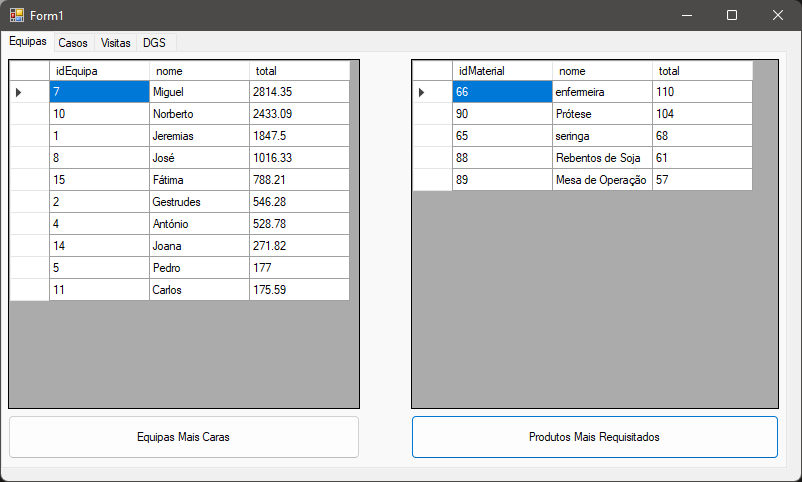
\includegraphics[scale=0.65]{imagens/EquipasDashboard.png}

\section{Visitas Diárias}

É necessário selecionar a tabela de fiscalização, separando as entradas inseridas no último mês.
De seguida é feito o calculo diário de visitas, e formatado de modo a apresentar numa tabela.

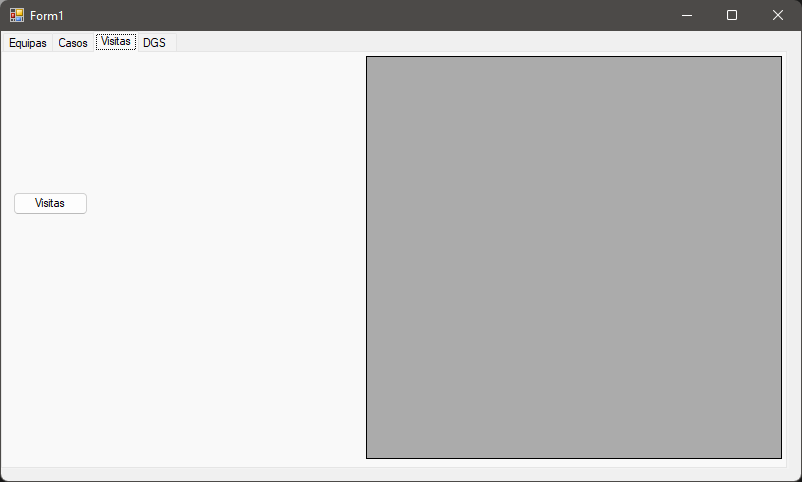
\includegraphics[scale=0.65]{imagens/VisitasDashboard.png}
\vfill
\section{Número Médio de Infetados}

Selecionando as tabelas de Casos, pesquisamos e escolhemos as entradas inseridas nos últimos meses.
De seguida é feito o calculo mensal de infeções e de seguida a média.

As tabelas são formatadas de modo a apresentar duas tabelas - Tabela de Casos Mensais e Tabela de Casos nos últimos 6 Meses.

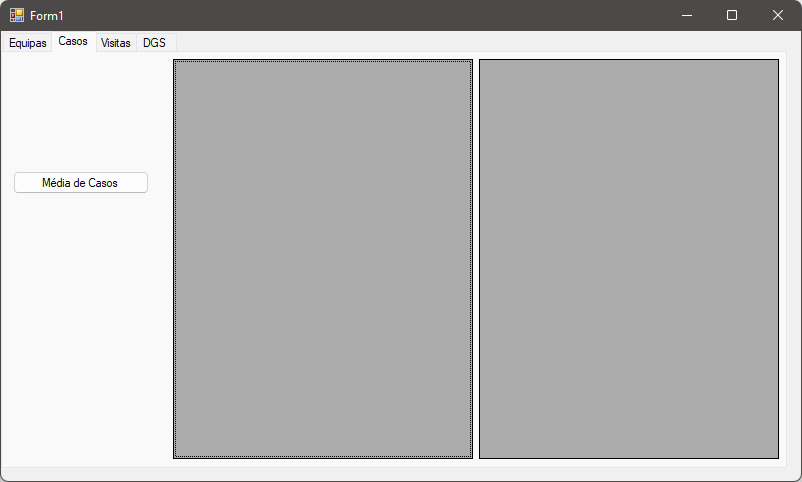
\includegraphics[scale=0.65]{imagens/CasosDashboard.png}
\vfill
\section{DGS}

Nesta secção são representados dados provenientes de uma API Rest cujo objetivo é mostrar dados sobre COVID em Portugal (https://covid19-api.vost.pt para documentação de rotas).
Os dados provenientes da request são formatados e apresentados no dashboard:

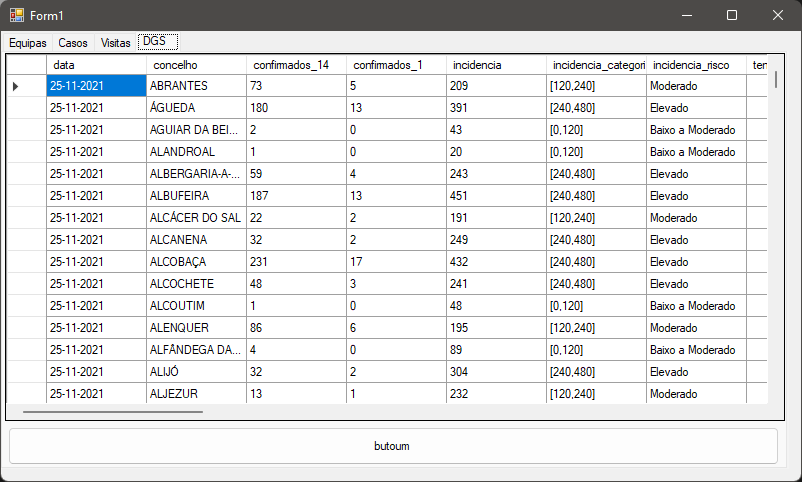
\includegraphics[scale=0.65]{imagens/DGSDashboard.png}